\chapter{Architektura systemu}

Dobre zaprojektowanie architektury systemu jest fundamentalnym zadaniem. Na rynku istnieje wiele infrastruktur opartych na technologii przetwarzania w chmurze, które oferują bardzo podobne funkcjonalności. Należało wybrać te, które dawały najwięcej korzyści przy jak najniższej cenie (kosztorys omówiono w rozdziale 3). Dlatego zdecydowano się na Microsoft Azure. Dodatkowym atutem było to, że zespół miał już doświadczenie z tą usługą. Opis działania poszczególnych elementów systemu zostanie omówiony w~dalszej części pracy.

\section{Schemat}

\begin{figure}[ht] 
   \centering
   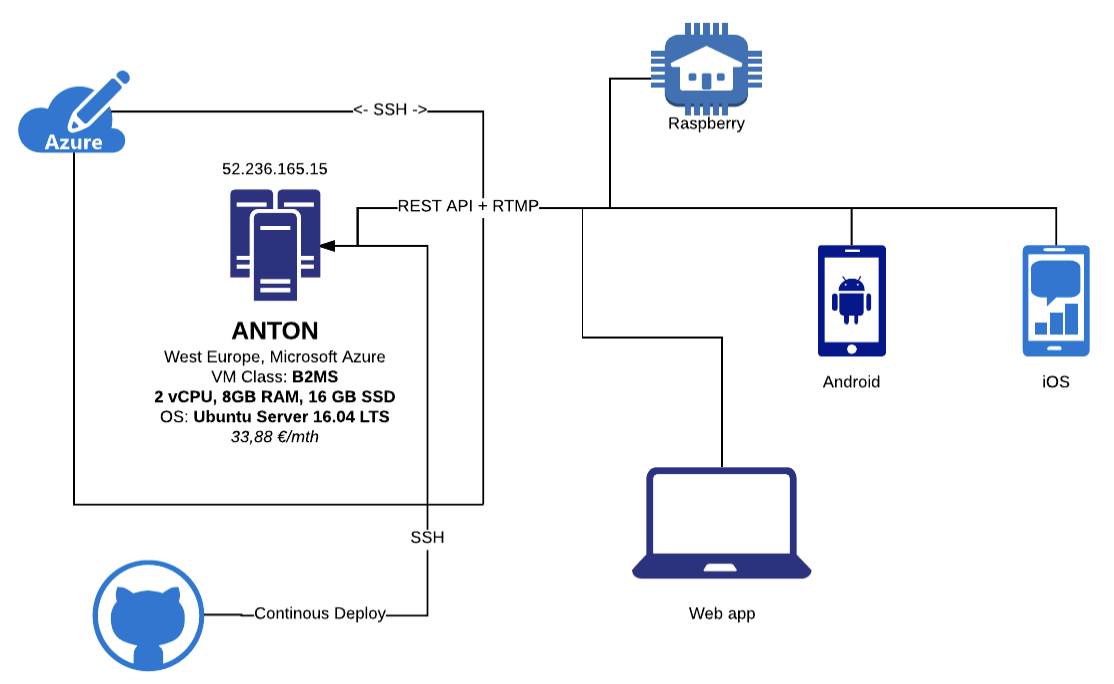
\includegraphics[width=12cm]{anton.png} 
   \caption{Schemat systemu [opracowanie własne]}
\end{figure}

Architektura została przedstawiona na schemacie (rys 2.1). Wszystkie urządzenia klienckie (iOS, Android i~Web), jak i~Raspberry Pi komunikują się z~serwerem ANTON wykupionym i~pracującym na platformie Microsoft Azure. Komunikacja pomiędzy klientami a~serwerem odbywa się dzięki REST API. Obraz natomiast przesyłany może być za pomocą dwóch protokołów RTMP i~HLS. Postanowiono, że transmisja obrazu w~systemie The Guard oparta będzie na protokole HLS ze względu na brak możliwości obsługi RTMP na iOS. Priorytetem było zapewnienie identycznych warunków i~tych samych doświadczeń użytkownika na wszystkich platformach. Było to głównym powodem całkowitego odrzucenia przesyłania obrazu przy użyciu protokołu RTMP. RTMP posiada jednak w~porównaniu do HLS jedną, aczkolwiek bardzo istotną przewagę. Jest to brak opóźnienia w~transmisji obrazu. HLS wysyła dane w~małych porcjach. Przed wysłaniem pierwszej części, konieczne jest jej nagranie. To właśnie powoduje kilkunastosekundowe opóźnienie w stosunku do RTMP, który transmituje obraz bezpośrednio. Oba protokoły omówiono dokładniej w~rozdziale 4.3.

\section{Komunikacja}

Komunikacja pomiędzy elementami systemu odbywa się na zasadach architektury REST. Wiadomości przesyłane są asynchronicznie, na wskazane wcześniej adresy.
Takie podejście gwarantuje prostotę przesyłanych komunikatów oraz skalowalność w~kontekście nowych urządzeń Raspberry strumieniujących dane oraz nowych urządzeń korzystających z~aplikacji klienckich. Początkowo projekt oparto o~zapytania GET i~POST.  \cite{WEBARCH}. Wprowadzenie tokenów uwierzytelniających (więcej w akapicie nt. Bezpieczeństwa) spowodowało, że wymianę komunikatów oparto tylko i~wyłącznie na zapytaniach POST. 

\paragraph{Zapytanie GET}
Metoda GET pozwala na pobranie dokumentu sieciowego, na postawie zapytania zawartego w~adresie URL. Metoda ta jest używana tylko i~wyłącznie do pobierania danych z~punktu docelowego. 

\paragraph{Zapytanie POST}
W metodzie POST, należy zamieścić wiadomość wewnątrz zapytania HTTP. Odpowiedzią na ten typ zapytania, może być zarówno kod statusu, jak i~dane, zwracane w podobnej postaci jak przy zapytaniu GET.

Wysłanie zapytania na określony adres powoduje uruchomienie specjalnej funkcji na serwerze. Każdy adres ma przypisaną osobną funkcję uruchamianą automatycznie po otrzymaniu zapytania. Funkcje te realizują operacje na bazie danych (CRUD) lub odpowiedzialne są za wysyłanie notyfikacji do wszystkich urządzeń klienta. Przykładowo (rys. 2.2) funkcja obsługująca dodanie nowego urządzenia w bazie danych, która uruchamia się po wysłaniu zapytania na adres /backend/v1/devices/add. Funkcja ta sprawdza czy zapytanie jest typu POST, pobiera przesłane dane i~wykorzystuje je do utworzenia nowego rekordu w~bazie danych.
\begin{figure}[ht] 
   \centering
   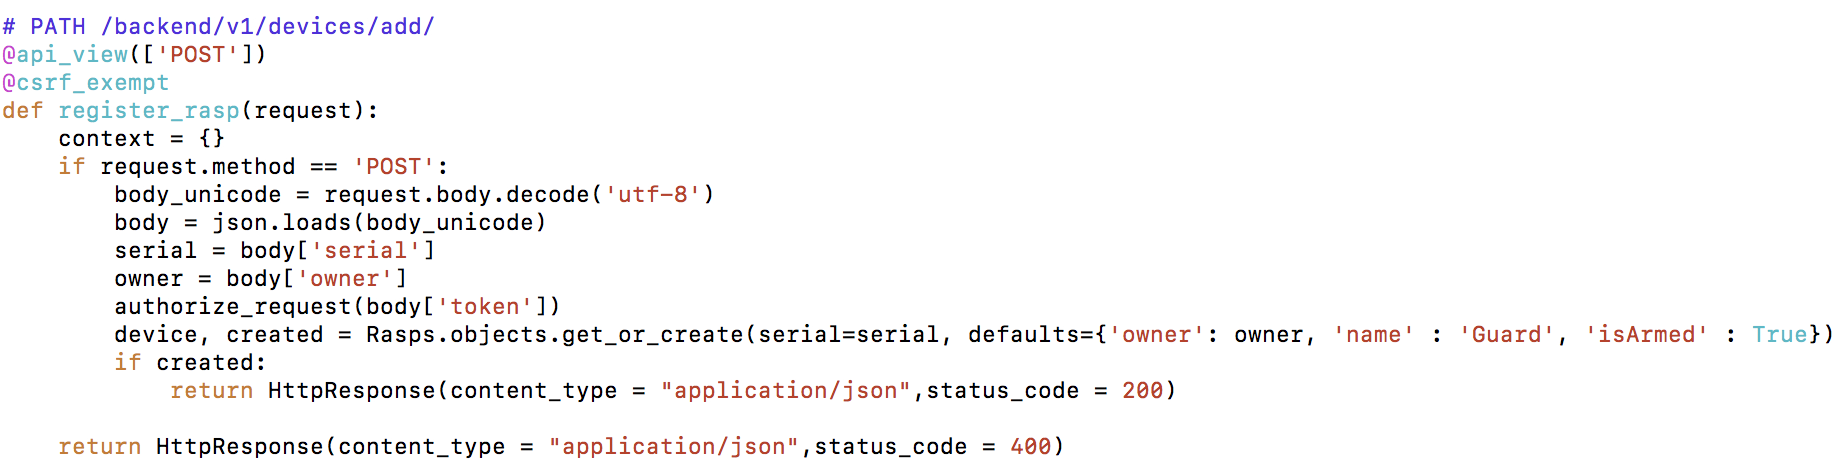
\includegraphics[width=14cm]{backend.png} 
   \caption{Funkcja obsługująca dodanie nowego urządzenia [opracowanie własne]}
\end{figure}

\section{Bezpieczeństwo}

Aplikacje wysyłając zapytania do serwera muszą potwierdzić swoją tożsamość. 
W aplikacjach mobilnych zastosowano proponowane przez Firebase rozwiązanie JSON Web Tokens. W~momencie wysłania zapytania POST do serwera, aplikacja dołącza także unikalny token generowany przez moduł Firebase Auth. Po dotarciu wiadomości do serwera, token ten weryfikowany jest przy użyciu modułu Firebase Admin SDK. Jeśli weryfikacja tokenów przebiegła pomyślnie (oba tokeny są identyczne) to udzielany jest dostęp do wykonania kodu na serwerze. W przeciwnym wypadku generowany jest błąd.

W~przypadku aplikacji internetowej zastosowano wbudowane w bibliotekę Django zabezpieczenia - przesyłanie tokenu CSRF oraz identyfikatora sesji wraz z~zapytaniem \cite{djangoCSRF}. Zabezpieczenie CSRF token uniemożliwia tzw. `Cross Site Request Forgery' tj. ataki w~których na stronie internetowej, bez wiedzy użytkownika uruchamiany jest skrypt (najczęściej w języku JavaScript). Następnie korzystając z~faktu, że użytkownik jest zalogowany strona atakująca podszywa się pod jego konto i~wysyła zapytanie do serwera, które może spowodować uruchomienie wszystkich operacji, do których upoważniony jest dany użytkownik. Aby tego uniknąć CSRF token zapisywany jest w~przeglądarce jako `ciasteczko' (eng. cookie) i dołączany do danych przesyłanych w~momenie wyboru przycisku odpowiedzialnego za przesłanie formularza. Wbudowana w~serwer Django biblioteka weryfikuje na podstawie zapisanych i~przesłanych danych sesji poprawność tokenu. W~przypadku błędu zwraca błąd serwera 403.
\\Ponieważ token przy każdym zapytaniu jest tworzony na nowo, na podstawie otwartej sesji pozostaje on rozwiązaniem przeznaczonym głównie dla aplikacji przeglądarkowych -~powyższe rozwiązanie nie byłoby komfortowe dla użytkowników aplikacji mobilnych: aplikacja musiałaby ustanowić połączenie z~serwerem (wysłać zapytanie GET na stronę główną) następnie zalogować się (wysłać zapytanie POST z danymi logowania) oraz zapisywać parę (token, id sesji) odsyłaną przez serwer. Aby ograniczyć ilość zapytań wysyłanych do serwera, w wypadku aplikacji mobilnych posłużono się inną opisaną powyżej metodą tokenów JWT.
